%%%%%%%%%%%%%%%%%%%%%%%%%%%%%%%%%%%%%%%%%%%%%%%%%%%%%%%%%%%%%%%%%%%%%%%
% Catching Misfiling in LLM Tool Narrators with Runtime Contracts Bound to Evidence
% V5: the 10 to 12 page paper, written for that length (not condensed).
% Every number comes from ../tse_latex/main.tex, the extended version, and is
% recomputed by the repository scripts; check_numbers.py verifies the overlap.
% Bibliography: references.bib, written by make_bib.py.
%%%%%%%%%%%%%%%%%%%%%%%%%%%%%%%%%%%%%%%%%%%%%%%%%%%%%%%%%%%%%%%%%%%%%%%
\documentclass[journal]{IEEEtran}

% IEEEtran asks for Times (ptm); under XeTeX's default TU encoding the font is
% not found and Latin Modern is substituted, so select the T1 encoding.
\usepackage[T1]{fontenc}
\usepackage{amsmath,amssymb,amsthm}
\usepackage{booktabs}
\usepackage{graphicx}
\usepackage[hidelinks]{hyperref}
\usepackage{url}
\usepackage{algorithm}
\usepackage{algpseudocode}
\usepackage{microtype}
\usepackage[htt]{hyphenat}
\tolerance=1200
\emergencystretch=1.5em

\renewcommand{\topfraction}{0.9}
\renewcommand{\bottomfraction}{0.6}
\renewcommand{\textfraction}{0.08}
\renewcommand{\floatpagefraction}{0.75}
\renewcommand{\dbltopfraction}{0.9}
\renewcommand{\dblfloatpagefraction}{0.75}
\setcounter{topnumber}{3}
\setcounter{bottomnumber}{2}
\setcounter{totalnumber}{5}
\setcounter{dbltopnumber}{2}

\graphicspath{{../tse_latex/}}
\newtheorem{definitionx}{Definition}
\hyphenation{mlcompass evi-dence-closed}

\begin{document}

\title{Catching Misfiling in LLM Tool Narrators\\
with Runtime Contracts Bound to Evidence}

\author{Hakan~Sabuni\c{s},
        Yusuf~\"Unl\"u,
        and~Mehmet~Kemal~\"Ozdemir% <-this % stops a space
\thanks{The authors are with the School of Engineering and Natural Sciences,
Istanbul Medipol University, Istanbul, T\"urkiye.
E-mail: hakansabunis@gmail.com (H.~Sabuni\c{s}), ysffms@gmail.com
(Y.~\"Unl\"u), mkozdemir@medipol.edu.tr (M.~K.~\"Ozdemir).}}

\markboth{Sabuni\c{s} \MakeLowercase{\textit{et al.}}}%
{Sabuni\c{s} \MakeLowercase{\textit{et al.}}: Catching Misfiling in LLM Tool Narrators}

\IEEEtitleabstractindextext{%
\begin{abstract}
Large language models (LLMs) increasingly narrate deterministic tool output,
and a narration can invent an item absent from that output or misfile a real
item into an inadmissible field. Prevailing defenses constrain decoding, which
needs token probabilities that commercial interfaces withhold, rely on
unobservable provider schemas, or check answers against pooled lists that pass
a real item in the wrong field. We propose evidence closed narration: every
answer field admits only tool output values bound at call time, numbers are
keyed to entity and statistic, and host code checks each answer. In the
assistant mlcompass, one of three LLMs failed often; 1,772 of its 1,831
violating answers used only items from the evidence, almost always the metric
name in a column field. A field description removed most such errors; a list written
for other data turned them into invention. Under the contract, no inadmissible
column or number reached the user through the structured fields, at
microseconds of local checking; an evidence bound enumeration did as well on
column names, and the check removed a small residue, 10 violations in
600, from the best configuration. We contribute an account of narrator failure,
a transferable design, and a registered guardrail comparison.
\end{abstract}

\begin{IEEEkeywords}
Tool use, faithfulness, hallucination, runtime verification, structured
output, guardrails, data leakage.
\end{IEEEkeywords}}

\maketitle
\IEEEdisplaynontitleabstractindextext
\IEEEpeerreviewmaketitle

%%%%%%%%%%%%%%%%%%%%%%%%%%%%%%%%%%%%%%%%%%%%%%%%%%%%%%%%%%%%%%%%%%%%%%%
\section{Introduction}\label{sec:intro}
%%%%%%%%%%%%%%%%%%%%%%%%%%%%%%%%%%%%%%%%%%%%%%%%%%%%%%%%%%%%%%%%%%%%%%%

\IEEEPARstart{L}{arge} language models (LLMs) increasingly stand between
deterministic tools and whoever consumes the tools' results. An agent calls a
tool, reads the structured output, and narrates what the output
means~\cite{react,toolformer,mcp}. The narration borrows the authority of the
tool, yet LLMs produce content that their input does not support~\cite{ji,huang}.
This paper studies faithful narration in the setting where the tool's output is
fully known at the moment of narration, and asks what that knowledge allows a
system to guarantee.

A leakage diagnosis illustrates the setting. A regression model that scores
$R^2=1.0$ on held-out data usually signals that the target has leaked into the
features~\cite{leakage}. In \textbf{mlcompass}, the open-source assistant for
machine-learning pipelines that serves as our testbed, a deterministic detector
measures how strongly each feature correlates with the target and ranks the
columns that may carry the target. An LLM, the \emph{narrator}, then explains the
detector's output, the \emph{evidence} $E$, in a structured answer: a verdict
(leakage likely, leakage uncertain, score legitimate, or cannot determine), the
columns cited as evidence, and claims of the form (column, statistic, value). On
our reference task, a sound answer cites the column \texttt{log\_target\_v2} and
its correlation of 0.999.

Without safeguards, one of the narrators that we tested listed \texttt{r2}
among the columns cited as evidence in 42\,\% of its answers. The string
\texttt{r2} is not a column but the name of the metric under investigation,
which $E$ carries for that reason, and the narrator's own prose treats
\texttt{r2} as the metric. The structured field, however, is the part that
programs consume, and mlcompass prints the field under the heading ``Evidence
cited (verified against the evidence)''. A reader would see a metric presented
as verified evidence, and a program would act on a column that does not exist.

This error is not the one that most defenses target. The narrator invented
nothing: the name is in $E$, in a field that does not admit the name. We call
such an error \emph{misfiling}, and an item that appears nowhere in $E$
\emph{invention}; in the vocabulary of Ji \emph{et al.}~\cite{ji} and Maynez
\emph{et al.}~\cite{maynez2020faithfulness}, they are intrinsic and extrinsic
errors. The two kinds call for different remedies: invention calls for grounding
the narrator in the evidence, misfiling for telling the narrator which field
admits what. They also differ in what detects them. A check that compares an
answer with the evidence as a pool of names and numbers passes a misfiled item
by construction, because the item is in the pool.

Existing defenses act in three places (Table~\ref{tab:taxonomy}). Constrained
decoding run by the caller restricts the tokens that a model may
emit~\cite{outlines,gcd,scholak2021picard} and needs token probabilities, which
commercial application programming interfaces (APIs) do not expose; providers
offer strict schema modes~\cite{structured} instead, whose enforcement cannot be
observed from outside. Validate-and-reask toolkits such as
Instructor~\cite{liu2023instructor} and Guardrails~AI~\cite{guardrailsai} check
the returned answer in the caller's code, with validators that may read
call-time context, and ask again when a check fails; which values each field
admits is left to the author of the validators, and a fresh installation checks
structure only. Recent checkers for narrations compare entities and numbers with
pools drawn from the evidence~\cite{gupta2026veritygate,du2026ledgermind}, which
accept a misfiled item.

For a narrator of a deterministic tool, which values each field admits has an
exact answer before the narrator is called: the columns, statistics, and values
that $E$ holds. We make that answer explicit. Admissibility is indexed by answer
field, and each number is keyed to the (column, statistic) pair whose value the
number claims to be. \emph{Tier~A} writes the admissible values of each field
into the JavaScript Object Notation (JSON) Schema of the narrator's answer tool,
as enumerations built from $E$ at call time, and \emph{Tier~B} checks the
returned answer in host code, sends the answer back with the violation named,
and deletes whatever still violates the contract. The enforcement mechanism is
ordinary validate-and-reask, available in the toolkits above, and we do not
claim the mechanism. We claim the granularity of the check, and what measuring
narrators at that granularity reveals. We ask three research questions.

\begin{itemize}
\item \textbf{RQ1}: How does an unconstrained narrator of tool evidence fail, and
which changes to its configuration remove the failure?
\item \textbf{RQ2}: What does the contract guarantee and cost, and how do the
alternatives in common use compare?
\item \textbf{RQ3}: Do the contract and the failure carry over to a second kind
of evidence?
\end{itemize}

We recorded 19{,}132 responses from three models on sixteen leakage tasks and a
dataset-profiling task, and 3{,}200 more in four registered, interleaved runs.
Only \texttt{deepseek-chat} failed often, and its failures were structural
misfiling: under the bare instruction, 1{,}772 of its 1{,}831 violating answers
used only items that $E$ contains, almost always \texttt{r2} in the cited-column
field, so a check against the pooled evidence would have passed them. One
sentence describing the field removed nearly all of these errors, whereas a
column list written for other data turned misfiling into invention: 145 of 200
answers cited columns that existed only in the list. Under the contract, no
inadmissible column or number reached the user through the structured fields in
any configuration that we ran, at microseconds of local checking. The comparison
also shows the limits of the check. On column names, an enumeration bound to $E$
did as well, and in the best configuration that we found, the check removed a
residue of 10 violations in 600 answers on the profiling task, a significant
difference that lies below the 5-point bar that our plan registered for
practical materiality.

The paper makes three contributions:
(i)~an empirical account of how a tool narrator fails when measured at the
granularity of answer fields: the dominant failure is structural misfiling,
which pooled checks pass and a field description largely prevents
(Section~\ref{sec:rq1});
(ii)~a transferable design for evidence-bound narration, with admissibility per
field and values keyed per pair, derived at call time and checked in host code,
together with the conditions under which the design applies
(Sections~\ref{sec:contract} and~\ref{sec:discussion}); and
(iii)~a registered comparison with the alternatives in common use that states
when each alternative suffices (Section~\ref{sec:rq2}). The replication
package~\cite{replication} holds every response, and an extended version of this
paper~\cite{extended} holds the full audit trail.

We do not claim that LLMs in general misfile rather than invent. The failure
occurred on one of three models, served under a rolling name, and centered on
one string. Our claim is narrower: when a narrator of tool evidence fails,
misfiling can dominate, a pooled check or a single hallucination rate would not
show the misfiling for what the misfiling is, and a check keyed to fields and
pairs catches both kinds of error.

%%%%%%%%%%%%%%%%%%%%%%%%%%%%%%%%%%%%%%%%%%%%%%%%%%%%%%%%%%%%%%%%%%%%%%%
\section{Background and Related Work}\label{sec:related}
%%%%%%%%%%%%%%%%%%%%%%%%%%%%%%%%%%%%%%%%%%%%%%%%%%%%%%%%%%%%%%%%%%%%%%%

\paragraph{Faithfulness to a finite record}
Data-to-text generation has long measured faithfulness against a finite input
record, with slot error rates~\cite{dusek2020e2e}, relation-generation
precision~\cite{wiseman2017challenges}, and table-grounded
metrics~\cite{dhingra2019parent}. Error typologies already separate kinds of
error: FRANK distinguishes entity errors from out-of-article
errors~\cite{pagnoni2021frank}, and Thomson and Reiter annotate wrong numbers,
wrong entities, and context errors~\cite{thomson2020gold}. Generators have also
checked their output against the input while decoding, by reranking candidates
for missing and redundant slots~\cite{wen2015sclstm,juraska2018slot}. In these
terms, a misfiled name or value is an entity or context error, or a wrong-value
slot, and an invented one is an out-of-article error. We borrow these categories
and claim neither them nor the idea of a check. What differs
for a tool narrator is the setting: the check must run on the payload that a
commercial API returns, without beams or token probabilities, before the user
sees the answer. Our evidence-closed assumption is a closed-world
assumption~\cite{reiter1978closed}. The enforcement is a postcondition in the
sense of Design by Contract~\cite{meyer1992dbc}, deleting what violates the
postcondition is suppression in the edit-automaton model~\cite{ligatti2005edit},
and Schneider~\cite{schneider2000enforceable} characterizes what a monitor can
enforce at all.

\begin{table}[!htbp]
\caption{Where a constraint on LLM output acts. \emph{Bound}: when the allowed
set is fixed, when the tool is written (author) or per request (call).
\emph{Logits}: whether the method needs token probabilities. \emph{Guarantees}:
what holds for every output. Our row shares its locus and binding time with
validate-and-reask tools; the difference is the granularity of the domain,
indexed by field and keyed by (entity, statistic) pair, against the pooled
domains of recent narration checkers.}
\label{tab:taxonomy}
\centering
\footnotesize
\setlength{\tabcolsep}{2pt}
\begin{tabular}{@{}p{1.9cm}p{1.5cm}p{0.78cm}p{2.1cm}p{1.82cm}@{}}
\toprule
Locus & Bound & Logits & Guarantees & Example \\
\midrule
Decode, grammar & author/call & yes & grammar & \cite{outlines,gcd,scholak2021picard,poesia2022synchromesh} \\
Decode, span & call & yes & verbatim spans & \cite{signe2026chyd} \\
Decode, closed loop & call & yes & none (empirical) & \cite{cruz2026atlasrtc} \\
Provider strict mode & author/call & no & the schema, if enforced (unobservable) & \cite{structured} \\
Code, policy & author & no & policy contract & \cite{ahn2026harness,zhang2025rvllm,winston2026solver} \\
Code, context + reask & call & no & what the validator checks & \cite{liu2023instructor,guardrailsai} \\
Code, ledger & accumulating & no & grounding in cited entries & \cite{du2026ledgermind} \\
Code, pooled gates & call & no & entity and number in the evidence pool & \cite{gupta2026veritygate} \\
Code, field-indexed & call & no & (C1)--(C2) per field and pair; (C3) flagged & this paper \\
\bottomrule
\end{tabular}
\end{table}

\paragraph{Where constraints act}
Decode-time methods can bind constraints to the input: grammar-constrained
decoding admits input-dependent grammars~\cite{gcd}, PICARD and Synchromesh check
partial programs against a database schema or a program's
scope~\cite{scholak2021picard,poesia2022synchromesh}, and
CHyD~\cite{signe2026chyd} restricts output to spans of the retrieved context.
All of them need token probabilities; ATLAS-RTC~\cite{cruz2026atlasrtc}
intervenes during decoding without a guarantee. What a schema enforces depends on
the engine that applies the schema~\cite{geng2025jsonschemabench}, and even the
wording of schema keys moves accuracy~\cite{le2026schemakey}. Instructor and
Guardrails~AI run validate-and-reask loops whose validators can read call-time
data, and NeMo Guardrails~\cite{nemo} applies output rails that block or rewrite
a response. Policy contracts fix their domain when the harness is written. Ahn
and Kim~\cite{ahn2026harness} find, as we do, that prompts let violations
through while enforcement in code keeps both safety and utility;
RvLLM~\cite{zhang2025rvllm} checks outputs against constraints written by
experts; and Winston \emph{et al.}~\cite{winston2026solver} compile policies
into solver constraints. Our contract has no domain until the evidence exists.
LedgerMind~\cite{du2026ledgermind} lets claims cite only active ledger entries,
checks entity and numeric grounding against the cited entries with a tolerance,
and restricts repair to edits that add nothing unprovenanced, our repair
asymmetry in another form; that ledger grows during a trajectory, whereas ours is
complete before the call. EviBound~\cite{chen2025evibound} gates a research agent
by querying the run tracker for the run that the agent claims.

\paragraph{Narration under a check}
Four recent works check what a model says about tool output.
FAX~\cite{kim2026fax} decomposes an agentic explanation into claims and tests
each claim against faithful tools before the final answer. Huang and
Deng~\cite{huang2026narration} show that in LLM-solver loops a verified verdict
can be inverted in narration, and that hardened prompts reduce but do not remove
the inversion; their channel is the verdict, which our contract leaves
unchecked. ProvenanceGuard~\cite{alvarez2026provenanceguard} targets claims that
are supported somewhere but attributed to the wrong source, which is misfiling at
the granularity of sources. VERITYGATE~\cite{gupta2026veritygate}, posted while
our runs were under way, is the closest in setting: four gates check that the
evidence identifiers of a narration exist, that each entity belongs to the set
that the backend emitted, that each number string matches exactly some number
string of the evidence, and that each claim type cites the evidence type that the
type requires. The entity and number gates compare with pools, so on evidence
like ours, whose pool contains the metric's name and every column's values, a
metric name in a column field and a neighbouring column's value would both
pass; the claim-type gate is a coarse form of field indexing. None of these works keys a number to the
entity and statistic that the number claims, or measures how often a failing
narrator misfiles rather than invents.

%%%%%%%%%%%%%%%%%%%%%%%%%%%%%%%%%%%%%%%%%%%%%%%%%%%%%%%%%%%%%%%%%%%%%%%
\section{Evidence-Bound Narration}\label{sec:contract}
%%%%%%%%%%%%%%%%%%%%%%%%%%%%%%%%%%%%%%%%%%%%%%%%%%%%%%%%%%%%%%%%%%%%%%%

\subsection{Evidence and admissibility}

In the leakage task, $E$ holds the suspicious metric and its value; the ten
features most correlated with the target, each with its correlation (whichever
of Pearson's and Spearman's coefficient is larger in magnitude, with its sign);
the ranked candidate leaks, the features whose correlation reaches 0.99 in
magnitude; and the rate at which predictions equal the target exactly.

\begin{definitionx}[Evidence-closed narration]\label{def:closed}
A narration task is \emph{evidence-closed} if the set of citable entities and
verifiable quantities is finite and machine-enumerable at the moment of the
narration call.
\end{definitionx}

Two simple checks suggest themselves for such a task. A check against the pool
of names in $E$, as the entity gates of recent checkers perform, passes
\texttt{r2}, because $E$ contains \texttt{r2} as the metric's name. A check
against the columns of the data frame rejects \texttt{r2} and invented names, but
admits real columns that the evidence does not support and says nothing about
numbers. We therefore index admissibility by field and key each number to a
pair, both derived from $E$ alone. The answer has two entity fields, the
cited columns (\texttt{columns\_referenced}) and the column of each claim
(\texttt{claims[].column}). From $E$ we derive the set $A_{E,\mathrm{col}}$ of
admissible columns and a table $V_E$ of measured values keyed by (column,
statistic). The \emph{anchor} $a^*$ is the top-ranked candidate leak, and an
answer \emph{commits} when its verdict is neither empty nor ``cannot determine''.

\begin{definitionx}[Evidence-bound runtime contract]\label{def:contract}
A structured response $r$ \emph{satisfies} $\mathcal{C}_E$, with tolerance
$\tau$, if \textbf{(C1, entity soundness)} every name in an entity field of $r$
lies in $A_{E,\mathrm{col}}$; \textbf{(C2, value soundness)} every claim
$(e,s,v)$ in $r$ with $e \in A_{E,\mathrm{col}}$ has $(e,s) \in
\mathrm{dom}(V_E)$, $v$ finite, and $|v - V_E(e,s)| \le \tau$; and
\textbf{(C3, anchor coverage)} if $r$ commits, $r$ references $a^*$.
\end{definitionx}

We call the three conditions the entity, value, and omission \emph{channels}.
An item is \emph{misfiled} when $E$ carries the item but not where the response
puts the item: a name of $E$ in an entity field that does not admit the name, or
a number of $E$ under a pair whose value the number is not. A name that $E$ does
not carry is \emph{unlisted} if the data frame has a column of that name and
\emph{invented} otherwise. The verifier sees only $E$ and treats all of these
alike; the distinctions serve measurement. Misfiling is a structural notion: a
misfiled item breaks the contract whether or not a reader would draw a false
conclusion from the item, and Section~\ref{sec:rq1} examines that question
separately.

\subsection{Two tiers and what they guarantee}

Fig.~\ref{fig:contract} and Algorithm~\ref{alg:contract} show the contract.
Tier~A writes $A_{E,\mathrm{col}}$ and the statistic names of $V_E$ into the
answer tool's schema as enumerations. An enumeration is a request to the model,
not a check: unless the provider enforces the schema during decoding, the model
may ignore the request. Tier~B therefore re-checks the returned answer in host
code for (C1) and (C2), with $\tau=0.005$, and for (C3). A violating answer goes
back to the model, at most twice, with the violation named. Whatever still
violates (C1) or (C2) after the retries is deleted, a cited name at a time or a
claim as a whole; an answer with no admissible verdict is aborted rather than
completed on the narrator's behalf. The deterministic evidence panel is printed
in every case, with the anchor first.

\begin{figure}[!htbp]
\centering
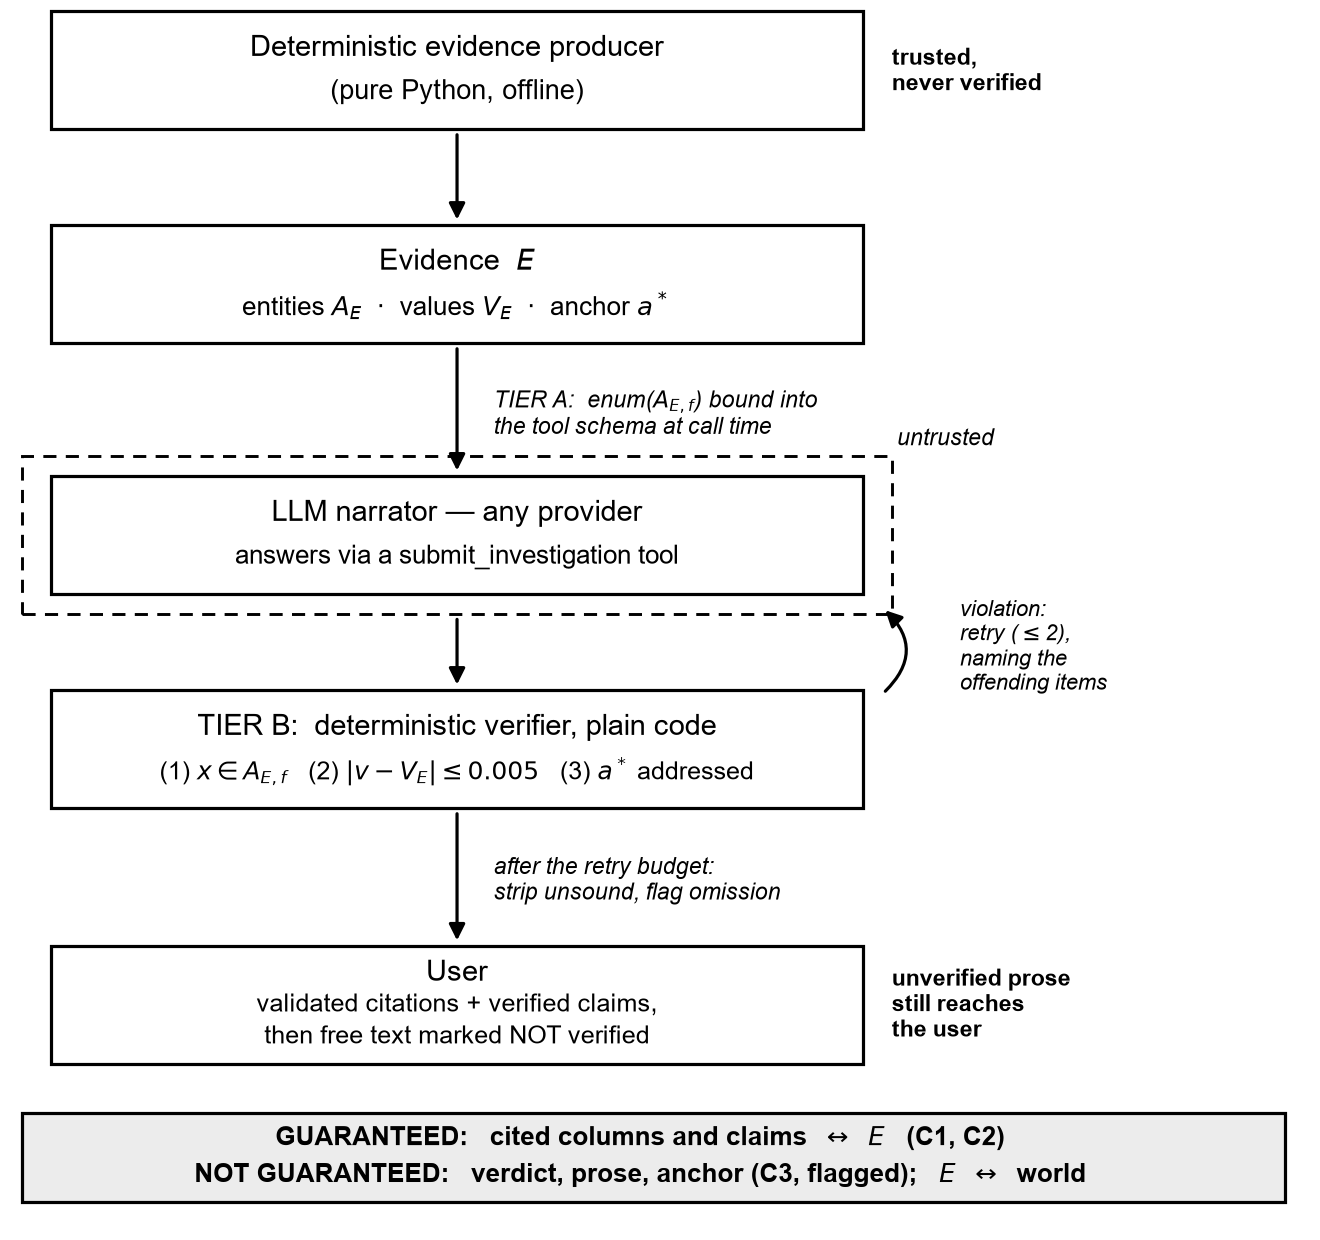
\includegraphics[width=\columnwidth]{fig1_contract.png}
\caption{The evidence-bound contract. Tier~A binds the answer schema's
enumerations to $E$ at call time. Tier~B re-checks the returned answer in host
code, retries with the offending items named, strips unsound content after the
budget, and flags a persistent omission. Only the narrator is untrusted; the free
text reaches the user marked unverified.}
\label{fig:contract}
\end{figure}

\begin{algorithm}[t]
\caption{Evidence-bound narration (budget $k=2$)}\label{alg:contract}
\footnotesize
\begin{algorithmic}[1]
\State $B \gets \mathrm{bind}(E)$ \Comment{$A_{E,\mathrm{col}}$, $V_E$, $\tau$, $a^*$}
\State $S \gets$ schema with enumerations from $B$ \Comment{Tier~A}
\State $c \gets$ empty correction
\For{$i = 0,\dots,k$}
  \State $r \gets \mathrm{model}(\text{prompt} + c, S)$
  \If{$r$ has no admissible verdict}
    \State $c \gets$ fixed correction; \textbf{continue}
  \EndIf
  \State $\mathit{viol} \gets \mathrm{verify}(r, B)$ \Comment{(C1), (C2), (C3)}
  \If{$\mathit{viol} = \emptyset$} \textbf{break} \EndIf
  \State $c \gets$ correction naming $\mathit{viol}$
\EndFor
\If{$r$ has no admissible verdict} \Return abort \Comment{evidence panel only}
\EndIf
\State $r \gets \mathrm{strip}(r, B)$ \Comment{drop names and claims violating (C1), (C2)}
\State $\mathit{flag} \gets r$ commits $\wedge\, a^* \notin \mathrm{refs}(r)$
\State \Return $(r, \mathit{flag})$ \Comment{(C3) flagged, never repaired}
\end{algorithmic}
\end{algorithm}

The contract therefore offers two different things: a guarantee for (C1) and
(C2), and a flag for (C3). Deletion makes (C1) and (C2) hold for every
structured claim that reaches the user, whatever the model does. The guarantee is a property of the design, so we
report an enforced arm's zero on these channels as what the verifier did and
attach no interval to the zero. (C3) is different. Deletion cannot repair a
missing anchor; any repair would add a reference that the model did not produce
and thereby fabricate attribution. Tier~B therefore only flags a persistent
omission, which is suppression without insertion~\cite{ligatti2005edit}. The
anchor check runs after stripping, because deleting a claim can orphan the
anchor.

\subsection{Implementation}

The contract is not tied to our code. Written for Instructor, the check is a
field validator that reads $E$ from the validation context and asks again on
failure~\cite{liu2023instructor}, at the same cost: one specification per
evidence shape. What the design contributes is what such a validator should
check, at which granularity, and the measurements that show why. In our
implementation, the contract is a layer that names no task. A specification of about forty lines
says how to read one evidence shape: which fields are entities, which
statistics each entity has, and which entity is the anchor. Leakage is one
specification; a dataset profiler is a second (Section~\ref{sec:rq3}). Checking an
answer costs $O(|r|)$, provided that $V_E$ is keyed on the pair (entity,
statistic): a table keyed on the entity alone checks a claim about one statistic
against another. Thirty-six hand-written mutation tests, ten fault-injection
tests that drive the shipped path with a narrator that repeats one fault, and a
registered property-based search over $10^6$ generated (evidence, response) pairs
support the implementation without proving the implementation correct. The
search, built after the experiments, found two defects: a NaN claim value passed
the verifier, and a 400-digit integer crashed the value check. Both are fixed;
the NaN fix came on 2026-09-24, after the main runs, and no recorded response
carries either value.

\subsection{What the contract does not cover}

The guarantee is consistency with $E$, not correctness. The verdict is checked
for admissibility but not for agreement with $E$, and the free-text narration
reaches the user marked unverified. The detector is trusted, so a mis-ranked
candidate is narrated faithfully. The contract governs one narration path: an
optional interpretation panel, a tool-server command whose client model narrates
in the user's editor~\cite{mcp}, and the \texttt{advise} command, which sends the
dataset profile to an LLM, run without the contract. Column names come from the
user's data, so a crafted header is a prompt-injection
vector~\cite{greshake2023injection}, and Tier~A writes that header into the
enumerations, the channel that EnumAttack uses to evade safety
training~\cite{zhang2025cda}. Rendered strings are escaped; nothing more is
guaranteed about them.

%%%%%%%%%%%%%%%%%%%%%%%%%%%%%%%%%%%%%%%%%%%%%%%%%%%%%%%%%%%%%%%%%%%%%%%
\section{Evaluation Design}\label{sec:design}
%%%%%%%%%%%%%%%%%%%%%%%%%%%%%%%%%%%%%%%%%%%%%%%%%%%%%%%%%%%%%%%%%%%%%%%

We evaluated the idea in a controlled experiment over fixed evidence, following
the ACM SIGSOFT Empirical Standards~\cite{ralph2020standards}, with mlcompass as
the testbed: the contract guards the leakage narration that the tool ships. The
manipulated variable is the enforcement mechanism, the instruction, or the
naming and description of the evidence; the outcome is what reaches the user.

\paragraph{Tasks}
The \emph{reference} task is a frame of 1,000 rows and fourteen columns whose
target $y\sim\mathcal{N}(50,10^2)$ has leaked through a log-transformed copy,
\texttt{log\_target\_v2}, alongside a highly correlated distractor; $E$ lists ten
columns. The \emph{crowded} task has 1,200 rows, the anchor \texttt{sensor\_ref}
at a correlation of 0.995, and nine near-tied distractors; none of its ten
evidence columns appears in the reference task. Two real datasets are explained
after an ordinary least-squares fit: \emph{bodyfat}~\cite{penrose1985bodyfat},
whose documented leak is \texttt{Density}, and
\emph{sambanis}~\cite{muchlinski2016civilwar}, a negative control with no
candidate. Twelve more tasks were frozen in the analysis plan on 2026-07-07,
before any live run: six target-derived leaks, each planted in two of four public
tables~\cite{lantz2013mlr,janosi1988heart,ibm2019telco,decock2011ames}. We wrote
the prompts, schemas, and contract against the reference task alone. The
profiling task of RQ3 is described in Section~\ref{sec:rq3}.

\paragraph{Narrators and sampling}
The narrators are \texttt{deepseek-chat}, \texttt{gpt-5.4-mini}, and a local
\texttt{qwen2.5:7b}, at temperature 1.0, the default of every endpoint and the
shipped setting. Each configuration ran 200 times per task on the hosted models
and 20 times on the local one; a count of 0 in 200 bounds the rate below 1.9\,\%
(Wilson, 95\,\%). The provider serves a rolling model name, so every rate carries
its run date, and we compare configurations within a date.

\paragraph{Configurations}
An \emph{arm} fixes the system prompt, the answer schema, and the check
(Table~\ref{tab:arms}). The \emph{bare} prompt states the task with no
faithfulness rule; the \emph{floor} is the bare prompt with an open schema and no
check. The \emph{shipped} prompt, the one mlcompass uses, adds seven rules and a
verdict mapping. The field description reads: ``Names of dataset columns
(features) from the evidence that you cite. Column names only, not the names of
metrics or statistics.'' Three arms share one Guardrails~AI loop and differ only
in the check: the stock validators, which check structure; our reimplementation
of the toolkit's acceptable-values semantics with the list built from $E$ (the
toolkit's own validator was not tested); and our checks. The two \emph{strong}
arms combine everything that helped (shipped prompt, call-time enumeration, field
description) and differ only in whether Tier~B runs. Every retry loop has a
budget of 2. The arms with a typed schema, \texttt{A-STRICT-ENUM}, and the lists
of A14 also sent the provider's \emph{strict} flag, which asks the provider to
enforce the schema during decoding. The harness sent the flag to the provider's
standard endpoint, whose documentation does not describe strict mode, and the
records show that the flag was not enforced (Section~\ref{sec:rq2}); no arm
therefore measured decoding enforced by the provider, and every enumeration in
this study acted as a request to the model.

\paragraph{Measures}
We score every delivered answer once into one table, from which every count is
computed (\texttt{scripts/unified\_scoring.py}). A violation is a breach of (C1),
(C2), or (C3); an answer \emph{flagged} on the entity channel cites at least one
inadmissible name. Each violating answer also receives one \emph{kind}, the first
that applies: \emph{extrinsic} (a name or number that $E$ lacks),
\emph{contradicts $E$} (for a pair that $E$ carries, the value of another item),
\emph{misplaced} (only items of $E$, in an inadmissible place), or
\emph{omission}. The middle two kinds are misfiling. The narrators copy numbers,
so the tolerance hardly matters: 22 answers carry a wrong number at every $\tau$
from $5\times10^{-4}$ to $0.01$. We report Wilson 95\,\% intervals with the raw
counts. Two scorers written independently from the definitions agree on every
entity flag across all 16{,}698 leakage records, and the seventeen faults that we
found in our own instruments changed derived numbers, never records; the extended
version lists them.

\paragraph{Registration}
The analysis plan and its amendments were frozen before the runs that they
govern. A result is \emph{confirmatory} only if the plan fixed its prediction
and test in advance; Table~\ref{tab:registered} lists the registered tests on
which the results below rest. The plan also registered a 2-point equivalence band
and a 5-point bar below which a significant difference is reported as not
material. When one arm has a verifier, the arm's zero on (C1) and (C2) holds by
construction, so a test against that arm asks whether the other arm's rate
exceeds zero. The remaining registered items were void (X2, H10: no non-entity
channel activated on leakage), not run or stopped (X5, H12, H15, A3~R1, R2b, R3,
R4, and the human audit A7), or are reported in the extended version (H7--H9,
H11, H13, H14, H16, A9.2, A10, A12). The deviations differ in weight. The stopped
A3 runs matter most, because the registered test of the verifier on the twelve
frozen tasks never ran; the model panel, changed without an amendment, limits
generality; the property-based search, built after the runs, tests the code but
not the runs; and X1, moved from the registered real-data task to the synthetic
one, is a control and carries no conclusion.

\begin{table}[!htbp]
\caption{Registered tests on which the results rest, strongest comparisons
first. Differences in percentage points (pp) with Newcombe 95\,\% intervals; X1,
X3, and X4 belong to the Holm-corrected family. X1 is a control: the stock loop
cannot reject \texttt{r2} by construction.}
\label{tab:registered}
\centering
\footnotesize
\setlength{\tabcolsep}{2pt}
\begin{tabular}{@{}lp{2.9cm}p{4.2cm}@{}}
\toprule
Item & Prediction & Outcome \\
\midrule
A11 & Verifier lowers violations in the best configuration & 10/600 against 0/600, $p=0.002$; 1.7 points [0.7, 3.0]; not material \\
A14 & Invented names fall with list coverage (P1) and stay above call time at 8 of 10 (P2) & 143, 2, 0, 3, 0 of 200: P1 holds ($p<10^{-76}$); P2 not supported ($p=0.25$) \\
X4 & Our checks in Guardrails tie the contract & 0.0\,pp [$-1.9$, 1.9], $p=1$; inside the band \\
X3 & Contract below a typed schema & 4.0\,pp [1.3, 7.7], $p_{\mathrm{Holm}}=0.015$; not material \\
A3 R2a & Invented names under 5\,\% of flagged answers on the 12 frozen tasks & Held: 12 of 817 (1.5\,\%) \\
A9.1 & More wrong numbers under suffixed names & 7 against 1 of 200, $p=0.068$; not significant \\
A13 & A stronger judge passes the validity check & Passed; misfiled \texttt{r2} read as false, 40/40 \\
X1 & Contract below the stock Guardrails loop & 35.5\,pp [28.9, 42.3], $p_{\mathrm{Holm}}<10^{-23}$ \\
\bottomrule
\end{tabular}
\end{table}

%%%%%%%%%%%%%%%%%%%%%%%%%%%%%%%%%%%%%%%%%%%%%%%%%%%%%%%%%%%%%%%%%%%%%%%
\section{RQ1: How the Narrator Fails}\label{sec:rq1}
%%%%%%%%%%%%%%%%%%%%%%%%%%%%%%%%%%%%%%%%%%%%%%%%%%%%%%%%%%%%%%%%%%%%%%%

\paragraph{The failure is misfiling}
On the floor, \texttt{deepseek-chat} cited an inadmissible name in 42.0\,\%
[35.4, 48.9] of 200 answers on 2026-09-15, and four runs over nine days read
42.0, 43.0, 40.5, and 49.0\,\% ($\chi^2$, $p=0.34$). On the first four tasks,
all 1{,}012 flagged answers of the arms without a column domain cited a name that
$E$ contains: \texttt{r2} in the list of cited columns, and three times
\texttt{perfect\_match\_rate}. The pattern is not an artifact of synthetic data.
The floor misfiled in 21.5\,\% [16.4, 27.7] of answers on bodyfat and 20.5\,\%
[15.5, 26.6] on sambanis, every time with \texttt{r2}. On the twelve tasks frozen
before any run, the floor cited an inadmissible name in 26.5 to 55.5\,\% of
answers per task, 817 of 1{,}888 in all: 795 misfiled, 18 cited only the frame's
own target column, which $E$ does not list, and 4 cited only an invented name,
so the registered prediction held. Across all sixteen tasks, 1{,}807 of the
1{,}829 flagged answers misfiled, and 13 used an invented name, some of them in
an answer that also misfiled; 11 of the 13 wrote \texttt{target} for the frame's
\texttt{y\_true}. These answers come from cells that differ in arm, task, and
date, so the composition describes the flagged answers rather than an error rate
over independent tasks. The failure is also narrow in form: almost every
misfiled name is \texttt{r2}. In the floor run of 2026-09-19, whose narrations
were recorded, 81 of 200 answers listed \texttt{r2} among the cited columns, 73
of them beside all ten evidence columns, and no narration called \texttt{r2} a
column. The narrator appears to read the undescribed field as a list of the
evidence that the narrator used, which makes the failure a property of the
interface as much as of the model.

\begin{table*}[!tp]
\caption{Kinds of violation; every answer is in exactly one row
(\texttt{deepseek-chat} unless named). \emph{Contract}: violates (C1), (C2), or
(C3), split by kind in the next four columns. \emph{Invented}: answers with a name
in neither $E$ nor the frame, a subset of the extrinsic ones. The four-task row
exceeds the 1{,}012 flagged answers by one omission and one wrong number; the
profile rows include the 93 and 91 answers of a stopped registered run (A3 R1);
the three \texttt{gpt-5.4-mini} violations are class-balance claims in 50 profile
probes. Generated by \texttt{scripts/unified\_scoring.py}.}
\label{tab:kinds}
\centering
\footnotesize
\setlength{\tabcolsep}{5pt}
\begin{tabular}{@{}lrrrrrrr@{}}
\toprule
Answers & $N$ & Contract & Extrinsic & Contradicts $E$ & Misplaced & Omission & Invented \\
\midrule
Leakage, bare instruction, four tasks & 3{,}200 & 1{,}014 & 1 & 1 & 1{,}011 & 1 & 1 \\
Leakage, bare instruction, twelve frozen tasks & 1{,}888 & 817 & 56 & 0 & 761 & 0 & 12 \\
Leakage, six instruction wordings & 600 & 370 & 21 & 1 & 348 & 0 & 20 \\
Leakage, field described or shipped prompt & 2{,}650 & 16 & 0 & 0 & 16 & 0 & 0 \\
Leakage, enumeration bound to $E$, no verifier & 600 & 0 & 0 & 0 & 0 & 0 & 0 \\
Leakage, enumeration written in advance & 800 & 152 & 145 & 0 & 0 & 7 & 145 \\
Leakage, Guardrails with choices or our checks & 1{,}400 & 3 & 0 & 2 & 1 & 0 & 0 \\
Leakage, contract arms & 4{,}000 & 0 & 0 & 0 & 0 & 0 & 0 \\
Profile, suffixed names, no verifier & 600 & 29 & 2 & 19 & 8 & 0 & 1 \\
Profile, natural names, no verifier & 693 & 36 & 14 & 0 & 22 & 0 & 14 \\
Profile, contract arms & 1{,}091 & 0 & 0 & 0 & 0 & 0 & 0 \\
\texttt{gpt-5.4-mini}, every arm & 1{,}450 & 3 & 0 & 0 & 3 & 0 & 0 \\
\texttt{qwen2.5:7b}, every arm & 160 & 2 & 2 & 0 & 0 & 0 & 2 \\
\bottomrule
\end{tabular}
\end{table*}

\paragraph{What the violations introduce}
Table~\ref{tab:kinds} assigns every violating answer to one kind. On the bare
leakage arms, 1{,}831 answers violate the contract, the 1{,}829 flagged answers
and two that breach only (C2) or (C3). Of these, 1{,}772 are misplaced, 57
extrinsic, one contradicts $E$, and one is an omission. Extrinsic answers dominate
in one place only, the enumeration written in advance for other data, where 145
of 152 violating answers name columns that the frame lacks; those names come from
the enumeration itself. On this model, most violations introduce nothing that $E$
lacks: the 1{,}772 misplaced answers use only items of $E$, so a check against the
pooled evidence would pass every one of them, and a contract rate read as a
hallucination rate would overstate invention many times over.

\paragraph{A semantic reading}
Whether a misfiled \texttt{r2} states a false relation is a semantic question. We
registered a blind human audit of 204 items (A7) and did not carry the audit out;
the sheet and its sampling script are in the replication package with the key
sealed. In its place we registered automatic judges, each with the same validity
check: at least 90\,\% correct in each direction on the items whose truth is fixed
by construction. Two natural language inference models (A10) and two LLM judges
(A12) failed. The fifth judge, \texttt{gpt-5.5} pinned to the snapshot of
2026-04-23 (A13), passed, keeping 55 of 55 items that are not false and catching
73 of 79 false or absent items (64 of 65 after correcting the strata for one
instrument fault). Contrary to our registered prediction that misfiled names
would read as right information in the wrong place, the judge classified all 40
misfiled \texttt{r2} items (Wilson interval 91--100\,\%) as false relations: a
cited column of that name asserts a column that the frame lacks. The validity
check, however, held no item whose true label is ``right information, wrong
place'', and the judge gave that label to no item, so the check cannot validate
the distinction on which this reading turns. We report one model's
classification, not a human judgment.

\paragraph{What a violation means}
Three quantities must therefore be kept apart. \emph{Structural violations} are
what the contract counts and enforces, by program, on every answer: 1{,}831 on
the bare leakage arms. \emph{Semantic falsehood} is what a reader would conclude;
the one validated judge read every audited misfiled \texttt{r2} as false, but the
reading is one model's and was not validated on the distinction at issue.
\emph{Correct content rejected} is the price of a closed world: all 15 real
columns that $E$ does not list were judged supported, and the contract rejects
them, and on the profiling task a correct class balance has no admissible slot
(Section~\ref{sec:rq3}). The contract guarantees the first quantity, bounds the
second only through the first, and pays the third.

\paragraph{What removes the failure}
The bare instruction says ``list every column from the evidence you cite'', and
the open schema says nothing about the cited-column field. A version of the
field description that names \texttt{r2}, run on the same day as the floor, and
the neutral description, run the next day, each took the rate from 49.0\,\%
(98/200, 2026-09-24) to 0.5\,\% [0.1, 2.8]. The arms were not interleaved, but the
drop far exceeds the floor's movement across four runs (40.5 to 49.0\,\%). The shipped prompt gave 0/200 with or without its two sentences claiming
that violations are rejected; its first three rules alone left 7.0\,\% [4.2,
11.4]; and temperature 0 left 2.0\,\% [0.8, 5.0]. Our names do not explain the
failure: on the crowded task, whose columns all differ, the undescribed field gave
61.0\,\% [54.1, 67.5], every time with \texttt{r2}. Nor does every model fail:
\texttt{gpt-5.4-mini} never wrote \texttt{r2} into a column field in 200 answers,
nor did \texttt{qwen2.5:7b} in 20. Six rule-free rewordings of the bare
instruction, 100 answers each, ranged from 9.0 to 72.0\,\%, as sensitivity to
prompt format would predict~\cite{sclar2024formatspread}, and the number of
claims on pairs that $E$ does not carry followed how much of the answer each
wording specified, from 0 per hundred to 45.

\paragraph{Answer to RQ1}
The failing narrator wrote the evidence's own vocabulary, above all \texttt{r2},
into an undescribed column field: 1{,}807 of 1{,}829 flagged answers misfiled,
13 used an invented name, and the misfiled answers would pass a pooled check.
The failure is structural and tied to the interface: a field description, the
shipped prompt, or temperature 0 lowered the rate from 42--49\,\% to 0--2\,\%
wherever we measured them.

%%%%%%%%%%%%%%%%%%%%%%%%%%%%%%%%%%%%%%%%%%%%%%%%%%%%%%%%%%%%%%%%%%%%%%%
\section{RQ2: What Enforcement Buys and Costs}\label{sec:rq2}
%%%%%%%%%%%%%%%%%%%%%%%%%%%%%%%%%%%%%%%%%%%%%%%%%%%%%%%%%%%%%%%%%%%%%%%

\begin{table*}[!tp]
\caption{Answers reaching the user with a violation (\%, 200 per cell,
\texttt{deepseek-chat}) and what reached the user on the reference task.
\emph{Date}: 2026 run date of the reference cell; the crowded task ran on
2026-09-24/25 and the strong arms on 2026-09-30. Below the second rule, the zero
on (C1) and (C2) holds by construction. \emph{Correct}: claims per answer that
match $E$. \emph{Retried}: answers sent back. Generated by
\texttt{scripts/unified\_scoring.py} and \texttt{scripts/delivery\_table.py}.}
\label{tab:arms}
\centering
\footnotesize
\setlength{\tabcolsep}{5pt}
\begin{tabular}{@{}lllrrrr@{}}
\toprule
Arm & Mechanism & Date & Reference & Crowded & Correct & Retried \\
\midrule
\texttt{A-L1} (floor)        & no enforcement                 & 09-15 & 42.0 & 61.0 & 9.6 & --- \\
\texttt{A-L1-T0}             & no enforcement, $T=0$          & 09-27 & 2.0 & --- & --- & --- \\
\texttt{A-GR-STOCK}          & Guardrails, structure only     & 09-15 & 35.5 & 57.5 & 9.8 & 0 \\
\texttt{A-STRICT-STATIC}     & typed schema, no column list   & 09-15 & 4.0 & 27.5 & 7.1 & --- \\
\texttt{A-STATIC-ENUM-STALE} & column list written in advance & 09-15 & 0$^{a}$ & 76.0$^{b}$ & --- & --- \\
\midrule
\texttt{A-L2}                & shipped prompt                 & 09-24 & 0 & --- & 2.2 & --- \\
\texttt{A-L2-RULES}          & its first three rules only     & 09-25 & 7.0 & --- & --- & --- \\
\texttt{A-L1-DESCRIBED-NEUTRAL} & field description           & 09-25 & 0.5 & --- & --- & --- \\
\texttt{A-TIER-A-ONLY}       & call-time enumeration          & 09-16 & 0 & 0 & --- & --- \\
\texttt{A-STRICT-ENUM}       & the same, strict flag          & 09-24 & 0 & --- & --- & --- \\
\texttt{A-GR-CHOICES}        & Guardrails, choices bound to $E$ & 09-18$^{c}$ & 0 & 1.5$^{d}$ & --- & 88 \\
\texttt{A-STRONG-NOVERIFY}   & shipped + enumeration + description & 09-30 & 0 & 0 & 3.1 & --- \\
\midrule
\texttt{A-GR-OURS}           & Guardrails, our checks         & 09-15 & 0 & 0 & 9.8 & 84 \\
\texttt{A-CONTRACT}          & Tier~A + Tier~B                & 09-15 & 0 & 0 & 9.7 & 0 \\
\texttt{A-STRESS}            & Tier~B alone                   & 09-15 & 0 & 0 & 9.7 & 12 \\
\texttt{A-L3-SHIPPED}        & as shipped, prompt included    & 09-24 & 0 & --- & 2.5 & 1 \\
\texttt{A-STRONG-CONTRACT}   & strong + Tier~B                & 09-30 & 0 & 0 & 2.9 & 0 \\
\bottomrule
\end{tabular}

\vspace{2pt}
{\footnotesize $^{a}$On the reference task the list equals the evidence's ten
columns.\quad $^{b}$152 of 200: 145 cite invented names, 132 of them also
omitting the anchor, and 7 more commit while citing nothing; 41 abstain.\quad
$^{c}$\texttt{A-GR-STOCK} read 43.5 that day.\quad $^{d}$3 of 200, in fields that
a single choice list does not check.}
\end{table*}

\paragraph{Every stated domain works on column names}
On the reference task, every arm that states the admissible columns reached zero
or one violation in 200, whether the shipped prompt, a field description, an
enumeration, a choice list inside a guardrail loop, or our verifier stated the
columns (Table~\ref{tab:arms}). On the entity channel, at this sample size, the
contract therefore does not outperform an enumeration or a choice list bound to
$E$, nor our checks inside another toolkit's loop (X4); any remaining distinction
rests on what each mechanism covers and certifies, not on the measured rate.
Because our checks matched the contract inside another loop, the contribution is
the check and its binding to $E$, not the loop. The enumerations, finally, acted
as requests. The list written for the reference task was sent with the strict
flag on the crowded task, and 13 of the 145 answers that cited columns from the
list also cited the anchor, which the list does not contain; decoding enforced
by the provider could not have produced them.

\paragraph{Stock guardrails check structure}
On 2026-09-18, the stock Guardrails loop and the same loop with a choice list
built from $E$ read 43.5\,\% against 0\,\%, with 88 answers sent back and
repaired. A fresh installation registers no faithfulness validator, so the stock
loop could not have rejected \texttt{r2}. On the crowded task, the choice list,
which checks only the cited columns, let three answers through, whereas our checks
in the same loop let none through (118 repairs). A typed schema without a column
list reached 4.0--7.0\,\% across runs, a significant but not material difference
from the contract (X3): schema text steers a model even where the schema
constrains nothing~\cite{le2026schemakey}.

\paragraph{Binding at call time}
A column list written in advance is the obvious alternative to binding at call
time, and on the reference task the two coincide. On the crowded task, the list
written for the reference task covers none of the ten evidence columns, and the
model obeyed the list: 145 of 200 answers (72.5\,\% [65.9, 78.2]) cited columns
that exist only in the list, an invention that the undescribed field never
produced, and 132 of them omitted the anchor, which the list does not contain.
The same task read 27.5\,\% with no list and 0\,\% with the list built at call
time. A registered, interleaved test then varied how stale the list is (A14):
lists covering 0, 3, 5, 8, or 10 of the ten evidence columns, each covering list
including the anchor, produced invented names in 143, 2, 0, 3, and 0 of 200
answers (Cochran--Armitage trend, $p<10^{-76}$). The trend is carried by the list
that covers nothing. At 8 of 10 columns, the residual could not be distinguished
from the call-time list at this sample size (3 against 0, Fisher $p=0.25$), and
because every covering list contained the anchor, the test does not separate the
anchor from the other columns. A list written in advance thus failed when the
list missed the evidence entirely, while a partly stale list that kept the anchor
behaved, at this resolution, like the list built at call time. Whether a list
written in advance is safe depends on a coverage that the list's author cannot
check before the data arrive; binding at call time removes that dependence.

\paragraph{The verifier in the best configuration}
The two strong arms read 0 in 200 on the reference, crowded, and both real
datasets on 2026-09-30, and the verifier never had to send a leakage answer back;
pooled over the four tasks, the difference is 0 with a Newcombe interval of $-0.5$
to 0.5 points. On the profiling task, an exploratory run left 4 of 200 unverified
answers in violation against none verified ($p=0.12$). We registered a
confirmatory test of both tasks (A3); both legs stopped when the provider balance
ran out, with no violation in their 93, 91, and 50 answers, and the registration
excluded repeating or extending that run. We therefore registered a new test on
the profiling task alone, before any call (A11): 600 answers per strong arm, one
call of each arm per index in a random order, on one harness commit, with every
attempt kept. One interim look at 358 unverified records (5 violating) is
recorded in the plan; no decision depended on the look. The unverified arm
delivered a violation in 10 of 600 answers (1.7\,\% [0.9, 3.0]) and the verified
arm in none, so the registered two-sided Fisher test rejects ($p=0.002$; difference
1.7 points, Newcombe interval 0.7 to 3.0). Two readings limit this result. First,
the whole interval lies below the 5-point bar that the plan set for practical
materiality, so by our own rule the difference is significant but not material;
A11 registered its own consequence, to report a benefit of the observed size, and
we read the result as a residue that the check removes at negligible cost, not
as a large improvement. Second, A11 does not exercise the value channel. The ten
violations are slips: two cite a statistic name as a column, four claim a pair
that $E$ does not carry, three of them under a statistic name that the profiler
does not use, such as the misspelled \texttt{missding\_count}, and four name a
column that the frame lacks. Nine of the ten fall outside the enumerations that
Tier~A writes, so an enumeration enforced by the provider would have refused
them too, and none is a wrong number for a carried pair. The verifier cost 11
extra calls in 600, and we saw no loss in what we measured: 29.4 correct claims
per answer in each arm, the anchor's value in every answer, and median latencies
of 5.47 and 5.44\,s.

\paragraph{Cost in time}
The local check and the call to the model differ in scale. Verification and
stripping take a median of 17\,$\mu$s per answer (95th percentile 41\,$\mu$s),
and binding $E$ takes 15\,$\mu$s. End to end, the contract arm took a median of
3.3\,s per answer against 2.8\,s for the floor; the difference comes from the
request, most likely the larger schema, and not from the check, although runs on
different dates cannot separate schema from provider. Retries add calls: one
named retry repaired every violation that the verifier met in the main runs, a
second retry was needed twice in 200 under a correction that names no problem
and once in A11, and arms that needed retries took 3.6 to 4.9\,s.

\paragraph{Content kept and content refused}
The check could buy compliance by emptying answers; the records show that the
check did not. All but one reference answer delivered at least one claim, none
abstained, and the contract arms delivered as many correct claims per answer as
the floor (Table~\ref{tab:arms}), as did both arms of A11. Nothing was ever
stripped in a live run, so deletion, the step that guarantees (C1) and (C2),
removed no content; how much a deletion would remove under real use therefore
remains unobserved. The retries rewrote answers without shedding correct
content: in a registered leakage re-run that kept every attempt (A9.2), the
retried answers carried 170 correct claims before the retry and 170 after, and a
script that shares no code with the verifier confirmed every rejection that the
records keep, 24 on the profiling task and 17 in that re-run. What the contract
refuses that is true, the price of the closed world, is counted in
Section~\ref{sec:rq1}. The arms with the shipped prompt, by contrast, delivered
about a quarter as many correct claims, so part of what that prompt buys is a
narrower answer.

\paragraph{Why Tier~B, not only enumerations}
An enumeration per field expresses the column domain, which is why the
enumeration arms tied the contract on leakage. The value channel is different:
the admissible value is a band around a number that depends on the column and
statistic chosen in sibling fields, and the anchor is a property of the whole
answer. Where a provider's strict mode supports alternatives, enumerations, and
numeric bounds, (C2) could be written as one branch per pair, a schema that grows
with $|V_E|$; we did not test such a schema, nor an enforced strict mode at all,
so the comparison is with enumerations as requests. Any such schema is enforced
inside the provider, whereas Tier~B checks the answer in our own process. We did
not compare against grammar-constrained decoding, because the one open model that
we ran did not fail without enforcement.

\paragraph{Answer to RQ2}
Under the contract, no (C1) or (C2) violation reached the user through the
structured fields in any configuration, a named retry repaired each violation,
and the local check costs microseconds. The alternatives fall into three groups.
A stock guardrail loop checks structure and does little. An enumeration or choice
list bound to $E$ matches the contract on column names. A list written for other
data turns misfiling into invention. In the best configuration that we found,
the verifier removed a residue of 10 violations in 600 answers on the profiling
task, significant but below our materiality bar, and none of the ten was a wrong
number for a carried pair. \texttt{gpt-5.4-mini} showed no violation in any of
the seven leakage arms that we ran on the model, so these comparisons rest on
\texttt{deepseek-chat}.

%%%%%%%%%%%%%%%%%%%%%%%%%%%%%%%%%%%%%%%%%%%%%%%%%%%%%%%%%%%%%%%%%%%%%%%
\section{RQ3: A Second Evidence Shape}\label{sec:rq3}
%%%%%%%%%%%%%%%%%%%%%%%%%%%%%%%%%%%%%%%%%%%%%%%%%%%%%%%%%%%%%%%%%%%%%%%

The second task is the deterministic dataset profiler that ships in the same
tool, bound through the same contract layer without a line of task-specific
verification. Its evidence has a different shape: every column of the frame is
admissible (24 against 10), each column has up to 13 statistics that depend on
its type (against 1), and $E$ carries 196 measured values (against 10). The frame
has ordinary data-quality problems and names its columns \texttt{num\_feature\_$k$}
and \texttt{cat\_feature\_$k$}, so a numeric and a categorical column share each
suffix; we also ran the frame under distinct natural names.

\begin{table}[!htbp]
\caption{The profiling task, 200 answers per arm, \texttt{deepseek-chat}.
\emph{C1}: an inadmissible column name. \emph{Wrong}: a number that misses the
measured value of its pair. \emph{N.c.}: a pair that $E$ does not carry.
\emph{Back}: answers sent back, for content / for an inadmissible verdict.}
\label{tab:rq6}
\centering
\footnotesize
\setlength{\tabcolsep}{2.6pt}
\begin{tabular}{@{}lrrrlr@{}}
\toprule
Arm & C1 & Wrong & N.c. & Any, \% [95\,\% CI] & Back \\
\midrule
\multicolumn{6}{@{}l}{\emph{Suffixed names (2026-09-19)}} \\
\texttt{P-L1} (floor) & 0 & 9 & 9 & 8.5 [5.4, 13.2] & --- \\
\texttt{P-TIER-A-ONLY} & 1 & 11 & 0 & 6.0 [3.5, 10.2] & --- \\
\texttt{P-CONTRACT} & 0 & 0 & 0 & 0 & 6/0 \\
\texttt{P-STRESS} & 0 & 0 & 0 & 0 & 13/0 \\
\multicolumn{6}{@{}l}{\emph{Natural names (2026-09-24; strong arms 2026-09-30)}} \\
\texttt{P-L1} (floor) & 8 & 0 & 20 & 13.0 [9.0, 18.4] & --- \\
\texttt{P-TIER-A-ONLY} & 5 & 0 & 1 & 3.0 [1.4, 6.4] & --- \\
\texttt{P-STRONG-NOVERIFY} & 3 & 0 & 1 & 2.0 [0.8, 5.0] & --- \\
\texttt{P-STRONG-CONTRACT} & 0 & 0 & 0 & 0 & 3/1 \\
\bottomrule
\end{tabular}
\end{table}

\paragraph{Misfiled values}
Here the failure moved from names to numbers (Table~\ref{tab:rq6}). Under
suffixed names, the floor put a wrong number in 9 of 200 answers (4.5\,\% [2.4,
8.3]), and 11 of its 12 wrong numbers are the real measurement of the column that
shares the suffix, such as \texttt{cat\_feature\_07}'s missing rate reported for
\texttt{num\_feature\_07}. Under natural names, five days later, the same model
put a wrong number in none of 400 unverified answers. A registered run that
interleaved the two naming schemes on one harness commit (A9.1) found 7 against 1
answers with a wrong number in 200 each ($p=0.068$), all seven suffixed ones
equal to the sibling's value. Name confusion is the likely explanation, but the
registered test did not reach significance, so the explanation remains
exploratory.

\paragraph{How the tiers separate}
The enumeration removed almost all claims on pairs that $E$ does not carry (20 to
1 under natural names), fewer inadmissible names (8 to 5), and no wrong numbers (9
against 11 under suffixed names). An enumeration can refuse a statistic that a
column lacks, but cannot constrain a number whose admissible value depends on
sibling fields. Tier~B caught both, and every contract arm read zero. A check
against the pooled evidence would not have: 11 of the 12 wrong numbers on the
suffixed floor, and all seven in A9.1, are numbers that $E$ carries for a
neighbouring column. This evidence is exploratory and comes from outside the
registered design. On leakage, the registered test of a channel that
enumerations cannot express was void (X2), the registered naming test did not
reach significance, and no host-filled or per-pair schema arm ran, so the claim
that only a pair-keyed check catches misfiled values holds among the arms that
ran. Most claims on
uncarried pairs are the class balance, which the profiler reports for the task as
a whole and the narrator attaches to the target column. The contract offers that
correct figure no slot, a design choice of ours; with the class shares admitted
on the target column, the floor falls from 26 to 10 violating answers under
natural names and from 17 to 10 under suffixed names.

\paragraph{Answer to RQ3}
The contract carried over to a second evidence shape without task-specific
verification. There the failure moved to misfiled values, which pooled checks
and enumerations pass and the pair-keyed check catches; the evidence for this
channel is exploratory.

%%%%%%%%%%%%%%%%%%%%%%%%%%%%%%%%%%%%%%%%%%%%%%%%%%%%%%%%%%%%%%%%%%%%%%%
\section{Implications}\label{sec:discussion}
%%%%%%%%%%%%%%%%%%%%%%%%%%%%%%%%%%%%%%%%%%%%%%%%%%%%%%%%%%%%%%%%%%%%%%%

\paragraph{Design principles for tool narrators}
Four principles follow from the measurements. We state them for narrators like
the one we studied, whose failure was structural; other models and tools may fail
differently. \emph{Check at the granularity of fields and pairs.} A check against
the pooled evidence would have passed 1{,}772 of the 1{,}831 violating answers
on the bare leakage arms, and 11 of the 12 misfiled values on the suffixed
profile frame. \emph{Bind the admissible sets at call time.} A list written for
other data turned misfiling into invention, and a list written in advance is safe
only to the extent of a coverage that the list's author cannot check.
\emph{Describe every field, and still check.} A one-sentence description was the
cheapest fix, and the description and the shipped prompt held wherever we
measured them, but the effect of such a fix is known only where the fix was
measured, whereas the effect of the check follows from code in the caller's
process; the residue that the check removed in A11 was small. \emph{Report
violations apart from what they introduce}, as data-to-text evaluation already
separates kinds of error~\cite{pagnoni2021frank,thomson2020gold}. A model judge
does not replace that report: four of the five judges that we tried failed a
90\,\% bar on items of known truth, and the one that passed costs about two cents
per item, against microseconds for the check.

\paragraph{Design alternatives}
Stripping without a retry would be cheaper, but would have deleted content from
6--16\,\% of \texttt{A-STRESS} answers and 41.5--59\,\% of the Guardrails arms'
answers, all of which one named retry repaired. Where the host renders the
answer, letting the model choose evidence identifiers while the host fills in
every number is preferable for the value channel, because the design removes
that channel by construction; the verdict, too, could be derived from $E$, which
would close the channel through which Huang and Deng show a verified verdict
being inverted~\cite{huang2026narration}. We ran neither design. The entity
fields and the anchor would still need a check, because an enumeration is a
request: 5 of 200 natural-name answers of \texttt{P-TIER-A-ONLY} put an
inadmissible name into a column field. A narrator whose output crosses a
tool-server boundary, finally, cannot have its numbers filled in by the host.

\paragraph{Beyond leakage}
The design needs a deterministic producer, a finite set of observed entities and
values, a domain bound to that set at call time, and a tolerance for each kind of
quantity; one absolute tolerance chosen for correlations can admit a neighbouring
value when two quantities lie close together. Narrators of static-analysis
findings, continuous-integration failures, or dependency-scanner reports meet
these conditions, although their evidence may be nested, relational, or larger
than ours. We have not measured them, and there, too, the guarantee would be
consistency with the tool's output, not correctness.

%%%%%%%%%%%%%%%%%%%%%%%%%%%%%%%%%%%%%%%%%%%%%%%%%%%%%%%%%%%%%%%%%%%%%%%
\section{Threats to Validity}\label{sec:threats}
%%%%%%%%%%%%%%%%%%%%%%%%%%%%%%%%%%%%%%%%%%%%%%%%%%%%%%%%%%%%%%%%%%%%%%%

\paragraph{Construct}
We measure consistency with $E$, not the effect of a narration on the decisions
of its readers; a contract violation is not always a false statement, and the
kinds are assigned by program (Section~\ref{sec:rq1}). Under one strict and one
lenient policy for dataset-level quantities, 98.7\,\% of the flagged bare leakage
answers misfile under every policy, whereas the lenient policy lowers the
unverified profile counts from 36 to 19 and from 29 to 22. No user study was run,
so the effect of a misfiled item on what a reader decides is not measured, and
no person labeled any
answer, and the semantic reading rests on one model's labels. The free text is
unverified; a scan
of 7{,}198 narrations found no clear displacement of ungrounded content into the
prose (8.8\,\% of narrations on reference arms that can reject a claim against
12.6\,\% on arms that cannot), but a misfiled name is in $E$ and so invisible to
that scan.

\paragraph{Internal}
Arms ran in blocks, except in the registered runs A9.1, A11, and A14, which
interleave their arms call by call, so drift within a day is controlled only
there. The provider serves a rolling model name and the harness changed between
runs; every record pins both, so a difference across dates cannot be attributed
to the provider alone.

\paragraph{External}
The failure occurred on one of three providers, at temperature 1.0, on particular
dates, and centered on one string, so every comparison rests on
\texttt{deepseek-chat} and on one evidence schema. No enforced strict mode, toolkit
validator of the toolkit's own, host-filled design, or producer outside mlcompass
was measured, and the conclusions are limited to the alternatives that ran. The
contract arms ran
on four of the sixteen leakage tasks and on the profiling task; on the twelve
frozen tasks, 512 of the floor's 2{,}400 calls were lost when the provider balance
ran out, each cell's last calls. The shipped default narrator,
\texttt{claude-opus-4-7}, was registered and not measured for lack of budget, and
on the real datasets we called the narrator directly, so we evaluate the
narration component rather than the product end to end. From 10 to 1{,}000
columns, the enumeration costs 38 bytes per column against 344 for the evidence;
provider limits on enumeration size are unmeasured.

\paragraph{Conclusion validity}
Two hundred answers to one evidence dictionary measure one configuration's rate,
not 200 tasks. At 200 answers per arm, a comparison against a zero arm reaches
$p<0.05$ at six events and detects a true rate of 4\,\% with power 0.8 but 2\,\%
with power of only 0.21, which bounds what the A14 comparison at 8 of 10 columns
could show; A11 used 600 answers per arm, enough to detect 1.5\,\% with power
0.89. Only the registered family is corrected for multiplicity.

%%%%%%%%%%%%%%%%%%%%%%%%%%%%%%%%%%%%%%%%%%%%%%%%%%%%%%%%%%%%%%%%%%%%%%%
\section{Conclusion}\label{sec:conclusion}
%%%%%%%%%%%%%%%%%%%%%%%%%%%%%%%%%%%%%%%%%%%%%%%%%%%%%%%%%%%%%%%%%%%%%%%

When an LLM narrates a deterministic tool's output, which values each field of
the narration admits has an exact answer at call time. We made that answer
explicit, at the granularity of fields and of (entity, statistic) pairs, and
measured three narrators against the answer. The one narrator that failed often
did not, for the most part, invent: 1{,}807 of its 1{,}829 flagged answers placed
an item that the evidence contains, above all the metric's name \texttt{r2}, in a
field that does not admit the item, a failure that a check against the pooled
evidence would pass and that a one-sentence field description removed where we
measured the description. A list of columns written for other data turned the
failure into invention. Checking every answer in host code at this granularity
let no inadmissible column or number reach the user through the structured
fields, behind an API that exposes no token probabilities, at microseconds of
local checking. The check is not the only mechanism that works: on column names,
an enumeration bound to the evidence did as well, and in the best configuration
that we found the check removed only a small residue. What the study contributes
is therefore less a new mechanism than an account of how a tool narrator fails
and a design that catches that failure wherever the configuration does not.
These results come from one failing model on one testbed, and the check does not
yet reach a client model that narrates the same evidence across a tool-server
boundary.

\section*{Acknowledgments}
We thank the readers of earlier drafts whose disagreement located a defect in our
value scorer.

% Declaration of AI-assisted tools (IEEE policy: disclosed in the
% acknowledgments, naming the system, the affected parts and the level of use).
% Keep this file in sync with the project record; edit here, not in main.tex.
\paragraph{Declaration of AI-assisted tools}
The authors used Claude (Anthropic), principally Claude Opus 5.5, accessed
through Claude Code during 2026. Claude drafted and revised manuscript text in
every section from the authors' notes, results and instructions, including a
final editing pass for readability; wrote and tested most of the measurement
harness, the analysis scripts that compute the reported tables, and parts of
the artifact's verification code; ran the experiment batteries under the
authors' direction; checked bibliographic entries against their sources;
simulated a multi-reviewer pre-submission review whose findings the authors
addressed; and built the sheet and the sampling script of the blind audit,
whose items the authors label themselves. The large language models \texttt{deepseek-chat},
\texttt{gpt-5.4-mini} and \texttt{qwen2.5:7b} are subjects of the study and
are described in Section~\ref{sec:design}. The authors chose the research
questions and the study design, reviewed and edited all text, inspected and
tested the code, recomputed every reported number from the released run
records, verified every reference, and made all analytical and interpretive
decisions. Claude is not an author, and the authors take full responsibility
for the content of this paper.


\section*{Data Availability}
The replication package~\cite{replication}, archived at
\url{https://doi.org/10.5281/zenodo.23025967} and developed at
\url{https://github.com/hakansabunis/mlcompass}, contains the artifact, every
harness, the frozen analysis plan with its amendments, one record per live
response with the verbatim reply delivered to the user, and the scripts that
recompute every table. Every record pins the commits of the harness and the
adapter under which the record ran; the tables are recomputed offline from the
records, without any call to a model, by \texttt{scripts/make\_tables.py},
\texttt{scripts/unified\_scoring.py}, and the scripts named in the captions; and
the dependency floors are declared in the package metadata. The extended
version~\cite{extended} reports the full audit
trail: every registered item with its timestamps and status, the instrument
faults, the free-text scan, and a downstream benchmark. Code is released under the
MIT license and data under CC-BY 4.0.

\bibliographystyle{IEEEtran}
\bibliography{references}

\end{document}
